%% Documentation for XPOMP
%% $RCSfile: xpomp_manual.tex,v $ (version $Revision$)
%% $Date: 1996/09/01 21:53:25 $, 

\documentclass[a4paper]{article}
\usepackage{psfig,xspace,html}
\begin{document}

\newcommand{\HPFC}{\htmladdnormallink{\texttt{hpfc}}
  {http://www.cri.ensmp.fr/pips/hpfc.html}\xspace}
\newcommand{\xPOMP}{\htmladdnormallink{\textbf{xPOMP}}
  {http://www.cri.ensmp.fr/pips/xpomp_manual/xpomp_manual.html}\xspace}
\newcommand{\POMP}{\htmladdnormallink{\textbf{POMP}}
  {ftp://ftp.ens.fr/pub/pomp}\xspace}
\newcommand{\POMPC}{\htmladdnormallink{\textbf{POMPC}}
  {ftp://ftp.ens.fr/pub/pompc}\xspace}
\newcommand{\HyperC}{\textbf{HyperC}\xspace}
\newcommand{\PIPS}{\htmladdnormallink{\textbf{Pips}}
  {http://www.cri.ensmp.fr/pips}\xspace}
\newcommand{\FC}{\htmladdnormallink{Fabien \textsc{Coelho}}
  {http://www.cri.ensmp.fr/people/coelho}\xspace}

%% Stack up all the figures and the text:
\renewcommand{\floatpagefraction}{1}
\renewcommand{\textfraction}{0}
\renewcommand{\topfraction}{1}
\renewcommand{\bottomfraction}{1}


\title{xPOMP: a Simple X11 graphical Library to Display Arrays in C,
  Fortran and HPF}
\author{Ronan \textsc{Keryell}\thanks{%
    \htmladdnormallink{Centre de Recherche en Informatique}
    {http://www.cri.ensmp.fr},
    \htmladdnormallink{�cole Nationale Sup�rieure des Mines de Paris}
    {http://www.ensmp.fr},
    35, rue Saint-Honor�,
    F-77305 \textsc{Fontainebleau cedex, France},
    \texttt{\htmladdnormallink{keryell@cri.ensmp.fr}
      {mailto:keryell@cri.ensmp.fr}}.}
  \and Nicolas \textsc{Paris}\thanks{%
    \htmladdnormallink{\textsc{ais} Berger-Levrault}
    {http://www.Berger-Levrault.fr},
    34, Avenue du Roul�, F-92200 \textsc{Neuilly sur Seine, France},
    \texttt{\htmladdnormallink{nico@Berger-Levrault.fr}
      {mailto:nico@Berger-Levrault.fr}}.}
  }

\maketitle

\section{Introduction}
\label{sec:introduction}

Visualization is a powerful tool to explore data but also to help
debugging programs, specially parallel programs where bugs are often
emphasized. \xPOMP is such a tool and can display 2-dimensionnal arrays
in XWindowS 11 windows as a part of the \PIPS project.

\xPOMP, like \HyperC from HyperParallel Technologies, is based on
previous work from the \POMP{}/\POMPC project at
\htmladdnormallink{�cole Normale Sup�rieure de
  Paris}{http://www.ens.fr}.



\section{User manual}
\label{sec:user}

From the user point of view, an \xPOMP window is a X11 window as shown
on Figure~\ref{fig:xPOMP_window}. It uses its own X11 colormap to
display a 256-level image.

\begin{figure}
  \begin{center}
    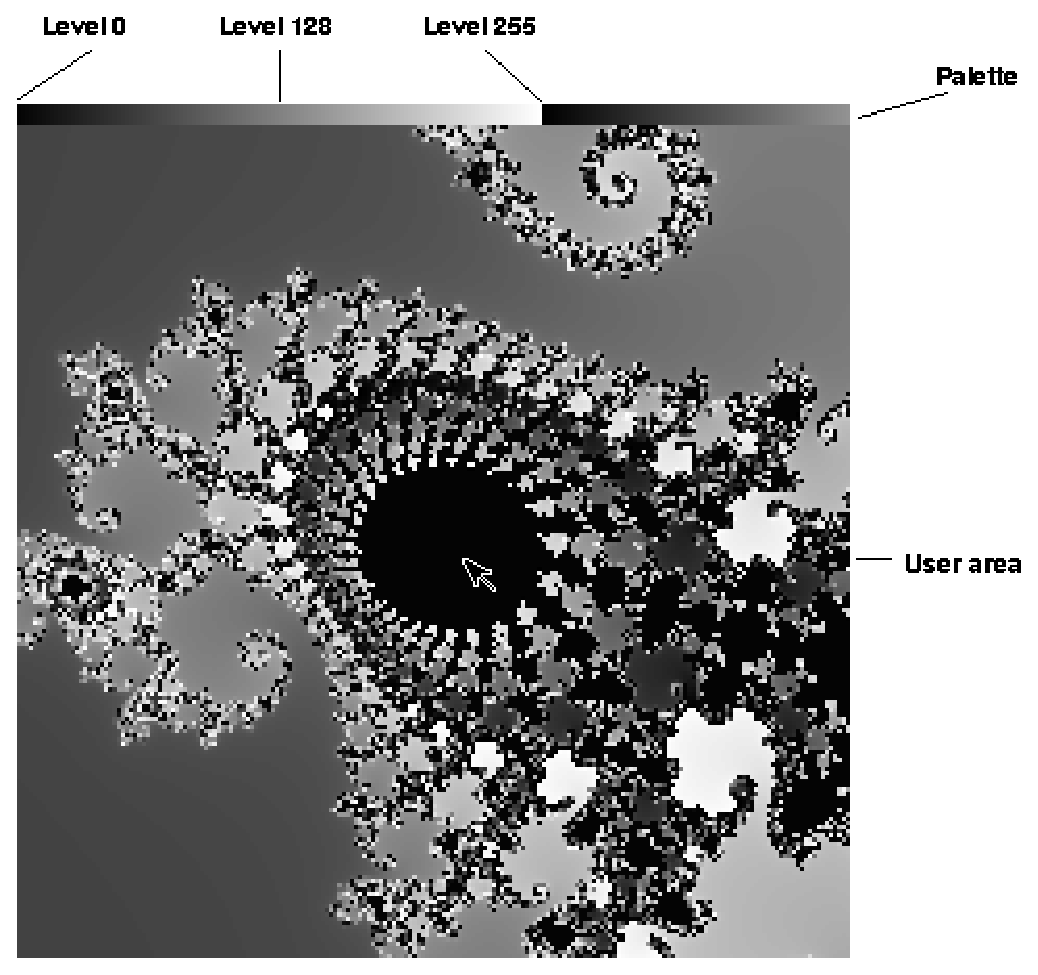
\psfig{file=xPOMP_window_explained.eps,width=\hsize}    
  \end{center}
  \caption{Example of an \xPOMP window displaying a fractal.}
  \label{fig:xPOMP_window}
\end{figure}

Such a window is splitted in 2 parts:
\begin{itemize}
\item a color map area that displays the colors scale from level 0 to
  level 255 from left to right. If the window width is less than 256,
  not all the color map is displayed but if the width is greater than
  256, the same color map is concatenated to fill the width ;
\item a user area where some arrays can be displayed, with the origin
  at the top left corner of the user area.
\end{itemize}

The mouse buttons can be used to send events to the application
program and the actions, if any, are defined by this application
program.

Many keystrokes can be used to control the \xPOMP viewer:
\begin{description}
\item[q or \^{}D:] quit the viewer window;
\item[color map type selection] ~
  \begin{description}
  \item[1:] grey scale;
  \item[2:] rainbow color;
  \item[3:] rainbow color with alternating half-tone. Useful to
    display small level differences;
  \item[4:] color centered, from blue to red. This color map is not
    linear and is useful to separate a small level zone;
  \item[0:] use the application defined color map if any;
  \end{description}
\item[color map parameters] ~
  \begin{description}
  \item[- or \_:] decrease the cycling rate of the color map;
  \item[+ or =:] increase the cycling rate of the color map;
  \item[h]: increase start value;
  \item[l:] decrease start value;
  \item[j:] decrease clipping level value;
  \item[k:] increase clipping level value;
  \item[H:] combination of 'h' and 'j' keys;
  \item[L:] combination of 'k' and 'l' keys;
  \item[?:] print out the actual color map parameters.
  \end{description}
\end{description}

\section{Programmer manual}
\label{sec:programmer}

An application program can open one or more \xPOMP windows to display
various numerical information. Each window can contain several array
image and the application program can get user feed back from the
mouse.

Each library function or procedure has 2 different definition
templates, one for the C language and another one for the Fortran
language. C function or procedure names begin with \verb|POMP_| but
Fortran ones begin with \verb|xpomp_|.

To declare the interface functions or procedures, one must include the
\xPOMP header file with
\begin{verbatim}
#include <xpomp_graphic.h>
\end{verbatim}
in C or
\begin{verbatim}
      include 'xpomp_graphic_F.h'
\end{verbatim}
in Fortran.



\subsection{Window manipulation}

\subsubsection{Opening a new window}

The first thing to do is to open a new \xPOMP window by calling the
function\\
C:
\begin{verbatim}
XPOMP_display window;
int X_window_size, Y_window_size;
window = XPOMP_open_display(X_window_size, Y_window_size);
\end{verbatim}
Fortran:
\begin{verbatim}
       integer window
       integer X_window_size, Y_window_size
       call xpomp_open_display(X_window_size, Y_window_size, window)
\end{verbatim}

This function open a window with a user area of size
\verb|X_window_size|$\times$\verb|X_window_size| and return a window
handler in \verb|window|.



\subsubsection{Closing a window}

The following procedures close the window connection
\verb|window|. Note that the \xPOMP window itself is not unmapped and
remain displayed.\\
C:
\begin{verbatim}
XPOMP_display window;
XPOMP_close_display(window);
\end{verbatim}
Fortran:
\begin{verbatim}
       integer window
       call xpomp_close_display(window)
\end{verbatim}



\subsection{Selecting a default display}

Most of \xPOMP routines can accept a display by default by giving them
the $-1$ handler value. If none default display exist, a new window is
created and it becomes the default window.

But the user can select a window as the default one by calling the
following functions that return the handler of the previous default
display if any or $-1$.\\
C:
\begin{verbatim}
XPOMP_display new_default_window, old_default_window;
old_default_window = XPOMP_set_current_default_display(new_default_window);
\end{verbatim}
Fortran:
\begin{verbatim}
       integer new_default_window, old_default_window
       call xpomp_set_current_default_display
      &    (new_default_window,old_default_window)
\end{verbatim}


\subsubsection{Getting the default window handler}

The default window handler (if any or $-1$) is returned by the following
functions:\\
C:
\begin{verbatim}
XPOMP_display default_window;
default_window = XPOMP_get_current_default_display();
\end{verbatim}
Fortran:
\begin{verbatim}
       integer default_window
       call xpomp_get_current_default_display(default_window)
\end{verbatim}


\subsubsection{Getting the display depth}

Since it may be useful to know the bit size of the window ixel to
display informations accordingly, this size is returned by:\\
C:
\begin{verbatim}
int depth;
default_window = XPOMP_get_depth();
\end{verbatim}
Fortran:
\begin{verbatim}
       integer depth
       call xpomp_get_depth(depth)
\end{verbatim}



\subsection{Displaying data}

\xPOMP can display array information in two way, one with character
type to directly control color or one with floating point type that is
mapped on the color color map.


\subsubsection{Displaying character array}
\label{sec:xpomp_flash}

The following functions display an unsigned character vector
considered as an array of size
\verb|X_data_array_size|$\times$\verb|Y_data_array_size| at position
$(\verb|X_offset|,\verb|Y_offset|)$ on the window \verb|window|. Each
pixel will have a size \verb|X_zoom_ratio|$\times$\verb|Y_zoom_ratio|.
The functions return 0 on success, $-1$ on failure. Each character
value directly control the color pixel through the color color map:
value 0 will be displayed with color map color 0 up to value 255
displayed with color map color 255. It is thus considered as an uncooked
mode.\\
C:
\begin{verbatim}
unsigned char * data_array;
int X_data_array_size, Y_data_array_size;
int X_offset, Y_offset;
int X_zoom_ratio, Y_zoom_ratio;
int status;
status = XPOMP_flash(window,
                     data_array,
                     X_data_array_size, Y_data_array_size,
                     X_offset, Y_offset,
                     X_zoom_ratio, Y_zoom_ratio);
\end{verbatim}
Fortran:
\begin{verbatim}
      integer window
      integer X_data_array_size, Y_data_array_size
      character image(0:X_data_array_size - 1, 0:Y_data_array_size - 1)
      integer X_offset, Y_offset
      integer X_zoom_ratio, Y_zoom_ratio
      integer status
      call xpomp_flash(window, data_array,
     &                 X_data_array_size, Y_data_array_size,
     &                 X_offset, Y_offset,
     &                 X_zoom_ratio, Y_zoom_ratio, status)
\end{verbatim}


\subsubsection{Displaying floating point array}

\xPOMP allows the representation of floating point array whose values
are mapped to color map color 1 to 254 (and not 0 to 255 to spare some
colors to be displayed as a clip layer or to detect overload). The
user given values \verb|min_value| and \verb|max_value| fix the value
matching color 1 and color 254. If the given values are both 0, these
values are set internally to the minimum and maximum values of array
elements.

Other parameters are the same as for Section~\ref{sec:xpomp_flash}.

Functions return $0$ when successful, $-1$ otherwise.

Since floating point value are often stored as single or double
precision that does not use the same memory storage, two different
interfaces exist.


\paragraph{Single precision interface}

\noindent
C:
\begin{verbatim}
XPOMP_display window;
float * image;
int X_data_array_size, Y_data_array_size;
int X_offset, Y_offset;
int X_zoom_ratio, Y_zoom_ratio;
double min_value, max_value;
int status;
status = XPOMP_show_float(screen, image,
                          X_data_array_size, Y_data_array_size,
                          X_offset, Y_offset,
                          X_zoom_ratio, Y_zoom_ratio,
                          min_value, max_value);
\end{verbatim}
Fortran:
\begin{verbatim}
      integer window
      integer X_data_array_size, Y_data_array_size
      real*4 image(0:X_data_array_size - 1, 0:Y_data_array_size - 1)
      integer X_offset, Y_offset
      integer X_zoom_ratio, Y_zoom_ratio
      integer status
      real*8 min_value, max_value;
      integer status
      call xpomp_show_real4(screen, image,
     &                      X_data_array_size, Y_data_array_size,
     &                      X_offset, Y_offset,
     &                      X_zoom_ratio, Y_zoom_ratio,
     &                      min_value, max_value, status)
\end{verbatim}


\paragraph{Double precision interface}

\noindent
C:
\begin{verbatim}
XPOMP_display window;
double * image;
int X_data_array_size, Y_data_array_size;
int X_offset, Y_offset;
int X_zoom_ratio, Y_zoom_ratio;
double min_value, max_value;
int status;
status = XPOMP_show_double(screen, image,
                           X_data_array_size, Y_data_array_size,
                           X_offset, Y_offset,
                           X_zoom_ratio, Y_zoom_ratio,
                           min_value, max_value);
\end{verbatim}
Fortran:
\begin{verbatim}
      integer window
      integer X_data_array_size, Y_data_array_size
      real*8 image(0:X_data_array_size - 1, 0:Y_data_array_size - 1)
      integer X_offset, Y_offset
      integer X_zoom_ratio, Y_zoom_ratio
      integer status
      real*8 min_value, max_value
      integer status
      call xpomp_show_real8(screen, image,
     &                      X_data_array_size, Y_data_array_size,
     &                      X_offset, Y_offset,
     &                      X_zoom_ratio, Y_zoom_ratio,
     &                      min_value, max_value, status)
\end{verbatim}


\subsection{Color Map operation}

Several type of color map exists and are named with the following
\verb|color_map_type| (note that they do not match their keyboard
accelerators):
\begin{description}
\item[0:] the grey shade color map
\item[1:] the rainbow color color map
\item[2:] rainbow color with alternating half-tone;
\item[3:] color centered, from blue to red;
\item[4:] use the application defined color map if any.
\end{description}


\subsubsection{Selecting a color map}

All the color maps but the application defined one are controled by the
following parameters:
\begin{description}
\item[cycle:] the color value evolved from one level to the next one
  as $2^\mathrm{cycle}$. Its value ranges from $-2$ to $6$;
\item[start:] is the level at which the color map cycling starts. Its
  value ranges from $0$ to $255$;
\item[clip:] is the level that is highlight. Its value ranges from $-1$
  to $255$. $-1$ stands for no highlight level.
\end{description}

C:
\begin{verbatim}
XPOMP_display window;
int color_map_type, cycle, start, clip;
int status;
status = XPOMP_set_color_map
    (window, color_map_type, cycle, start, clip);
\end{verbatim}
Fortran:
\begin{verbatim}
      integer window
      integer color_map_type, cycle, start, clip
      integer status
      call xpomp_set_color_map
     &    (window, color_map_type, cycle, start, clip, status)
\end{verbatim}

Note that when selecting \verb|color_map_type| 4 (that is the user
defined on, see Section~\ref{sec:selecting_user_colormap}), other
color map parameter values are not taken into account.

These functions return 0 on success and $-1$ otherwise.

\subsubsection{Selecting a color map}

The application can defined each color of all the 256 level by giving
three array values for the red, green and blue component.\\
C:
\begin{verbatim}
XPOMP_display window;
char red[256], green[256], blue[256];
int status;
status = XPOMP_set_user_color_map(window, red, green, blue);
\end{verbatim}
Fortran:
\begin{verbatim}
      integer window
      character red(256), green(256), blue(256)
      integer status
      call xpomp_set_user_color_map
     &    (window, red, green, blue, status)
\end{verbatim}

These function implicitly select the user defined color map.

These functions return 0 on success and $-1$ otherwise.


\subsection{Mouse interface}

The application program can get mouse button clicks in a blocking or
non-blocking way. The number of the button (usually 1 for left button,
2 for middle button and 3 for right button) pressed and the position
$(\verb|X|,\verb|Y|)$ of the cursor in the user area are returned by
the following functions.


\subsubsection{Waiting for a mouse click}
The following functions block up to the user click with the mouse
somewhere in the window:
C:
\begin{verbatim}
XPOMP_display window;
int button;
int X, Y;
button = XPOMP_wait_mouse(window, &X, &Y);
\end{verbatim}
Fortran:
\begin{verbatim}
      integer window
      integer button
      integer X, Y
      call xpomp_wait_mouse(window, X, Y, button)
\end{verbatim}


\subsubsection{Test for a mouse click}
The following functions just test for a user click with the mouse
somewhere in the window and do not block:
C:
\begin{verbatim}
XPOMP_display window;
int button;
int X, Y;
button = XPOMP_is_mouse(window, &X, &Y);
\end{verbatim}
Fortran:
\begin{verbatim}
      integer window
      integer button
      integer X, Y
      call xpomp_is_mouse(window, X, Y, button)
\end{verbatim}

If there is no mouse press down event, the value 0 is returned instead
of the button number.

\subsection{Display \xPOMP usage}

It is useful for an application to display a small description of the
keyboard usage of \xPOMP. This can be done by calling the following
procedures.\\
C:
\begin{verbatim}
XPOMP_display window;
int button;
int X, Y;
button = XPOMP_is_mouse(window, &X, &Y);
\end{verbatim}
Fortran:
\begin{verbatim}
      integer window
      integer button
      integer X, Y
      call xpomp_is_mouse(window, X, Y, button)
\end{verbatim}


%%% PIPS/HPFC/XPOMP

\section{Using the xPOMP interface with HPFC}

\HPFC is the HPF prototype compiler included in the \PIPS project.
It is developped by \FC. In order to compile an HPF program which uses
\xPOMP, convinient headers, functions and extensions are provided.


\subsection{XPOMP/HPFC headers}

Firstly headers are provided (\verb|xpomp_graphics_F.h| file) that must be
included by all user HPF functions or subroutines that make use of the
\xPOMP library. This header file simply lists the subroutines and
declares them as I/O routines to the \HPFC compiler through the special
\verb|io| directive:
\begin{verbatim}
!fcd$ io xpomp_show_real4
!fcd$ io xpomp_is_mouse
\end{verbatim}
%%
The effect is that a special compilation scheme is
used for handling these functions and subroutines: they are called
by the \emph{host} processor only, after a collect of the needed data.
Data modified within subroutine are updated on the node
processors after the call. The compiler figures out these effects 
thanks to the interprocedural analyses and the \emph{fake} routines
provided, as described in the next section.


\subsection{Fake functions}

As \PIPS is an interprocedural compiler, fake functions sources
for the \xPOMP routines (\verb|xpomp_fake.f| file)
that simply mimic their effects on arguments are provided. 
They must be compiled together with the HPF program through \PIPS in
order to provide the compiler with the necessary information for
using the \xPOMP display facilities. All \xPOMP functions are annoted
as \verb|io| and\verb|fake| with special \verb|!fcd$| %% $
(\FC directives). The first directive tells that the function or
subroutine performs only I/O. 
The second directive tells that the source provided are fake. The effect is
that the compiler will not generate code by compiling the functions, but
they will have to be provided at link-time.
%%
The \verb|hpfc| front end accepts
a list of files for compilation, hence for compiling the \verb|fractal|
exemple one must write:
\begin{verbatim}
    hpfc xpomp_fake.f fractal.f
\end{verbatim}

\subsection{Linker extensions}

Since the source files for the functions are fake ones (the functions
are actually written in C), these functions must be provided latter on
at link-time. The \HPFC compiler allows to give this information
with the \verb|!ldi$| %%$
(Link eDitor I/o) special directive. This directive supplies aditionnal
\verb|ld| options for linking the program with an I/O library (hence
the library is just linked to the \emph{host} program.
Assuming the \xPOMP library and executables being stored in
a directory described by the \verb|$XPOMP_RUNTIME| environment
variable, then the desired effect is achieved with: 
\begin{verbatim}
!ldi$ -L$XPOMP_RUNTIME -lxpomp
\end{verbatim}
Note that the variables are interpreted by a shell. This directive
is incorporated in the fake sources file for \xPOMP.

\newpage
\tableofcontents

\end{document}
